\documentclass[12pt,a4paper]{article}
\usepackage{tpl}
\dbegin{Кружок 7 класса, продолжающие, школа 179}{Решения занятия 17}

\z Есть кран с водой и цилиндрическая кастрюля. Как набрать ровно половину кастрюли?

\s Наклоним кастрюлю так, как показано на рисунке ниже, и нальём воду до границы. Это будет ровно половина кастрюли.\QEDA\\

\z Винни-Пух и Пятачок одновременно отправились в гости друг к другу, но, всю дорогу считая пчел, не заметили друг друга при встрече. После встречи Пятачок подошел к дому Пуха через 4 минуты, а Пух к дому Пятачка через минуту. Сколько минут был в пути каждый из них?

\s Пусть Пух идёт быстрее Пятачка в $k$ раз. Тогда точка встречи ближе к дому Пятачка в $k$ раз, значит, после встречи Пух потратит в $k^2$ раз меньше времени. Значит, $k^2=4$, откуда $k=2$. Значит, Пух шёл 3 минуты, а Пятачок 6.\QEDA\\

\z Гном Шоппин потратил 37 талеров, использовав монеты по 3 и 5 талеров. Какое наименьшее количество монет он мог использовать?

\s Заметим, что если монет минимальное количество, то монет по 5 максимальное, и больше 5 их взять не получится ($37-30=7$ и $37-35=2$ не делятся на 3, а $40>37$). Ответ: 9 монет. \QEDA\\

\z Вася задумал четырехзначное число. Когда он разделил это число на 119, в остатке получилось 115, а когда разделил его на 120, в остатке получилось 99. Какое число задумал Вася?

\s Заметим, что 2019 подходит. С другой стороны, если какие-то два числа подходят, то их разность делится на 119 и на 120, т.е. делится на какое-то пятизначное число ($119\cdot120$), значит, оба числа не могут быть 4-значными.\QEDA\\

\z Если бы Заяц стоял на месте, то Волк добежал бы до него за 4 минуты. Зайцу до домика бежать 6 минут в противоположную от Волка сторону. Волк бегает в два раза быстрее Зайца. Успеет ли Заяц добежать до своего домика раньше, чем Волк его догонит?

\s Зайцу до текущего места, где стоит волк, бежать 8 минут, а до домика 6 минут. Значит, если бы волк бежал со скоростью зайца, он бежал бы 14 минут, а с его собственной скоростью 7 минут. Значит, заяц спасётся.\QEDA\\

\z Есть 10 мешков с монетами, в каждом по 100 монет. Один из мешков целиком заполнен фальшивыми монетами, которые на 1 грамм легче настоящих. Чашечные весы со стрелкой показывают, на сколько граммов левая чашка легче или тяжелее правой. За одно взвешивание определите фальшивый мешок.

\s Положим на левую чашку весов 1 монету из 1-го мешка, 2 монеты из 2-го мешка, \ldots, 9 монет из 9-го мешка, на правую --- 45 монет из последнего мешка. Если перевесила левая, то фальшивый мешок последний, иначе номер мешка равен разности между чашками (в граммах). \QEDA\\

\z Легко разместить комплект кораблей для игры в <<Морской бой>> на доске $10 \times 10$. А на какой наименьшей квадратной доске можно разместить этот комплект? (Комплект кораблей состоит из: одного корабля $1 \times 4$, двух --- $1 \times 3$, трех --- $1 \times 2$ и четырех --- $1 \times 1$. Согласно правилам корабли не должны соприкасаться даже углами.)

\s Пример на $7\times7$ нарисован ниже. $6\times6$ не хватает, потому что в каждом узле сетки должен быть максимум 1 корабль, и у этих кораблей суммарно 50 узлов.\QEDA\\
\newpage

\z Есть две кучи по 11 камней. Двое по очереди берут камни, за ход можно взять один камень из любой кучи или по одному камню из каждой кучи. Проигрывает тот, кому нечего брать. Кто из игроков (начинающий или его противник) может всегда побеждать и как ему играть?

\s Выигрывает первый. Стратегия такая: вначале взять один камень из каждой кучи, а потом копировать ход оппонента. После хода оппонента в тех кучах, откуда он только что взял камень, будет нечётное число камней, а значит, будет хотя бы один и скопировать ход получится, тогда опять во всех кучах станет чётное количество камней.\QEDA\\

\z Прямоугольник разрезали шестью вертикальными и шестью горизонтальными разрезами на 49 прямоугольников. Оказалось, что периметр каждого из этих прямоугольников --- целое число метров. Обязательно ли периметр исходного прямоугольника --- целое число метров?

\s Заметим, что суммарный периметр прямоугольников, лежащих вдоль большой диагонали (находящийся в левом верхнем углу, второй сверху и второй справа, \ldots, находящийся в правом нижнем углу), равен периметру исходного прямоугольника. Все эти периметры целые, значит, периметр исходного прямоугольника также целый.\QEDA\\

\n Придумайте пять различных натуральных чисел, произведение любых двух из которых делится на сумму этих пяти чисел.

\s Возьмём числа $15,30,\ldots,75$. Их сумма равна $15^2$, а т.к. каждое из них делится на $15$, то произведение любых двух делится на $15^2$.\QEDA

\p Можно ли придумать 100 чисел с аналогичным свойством?

\s Пусть $a=\frac{100\cdot101}2=5050$. Тогда по аналогичным причинам числа $a,2a,\ldots,100a$ подходят.\QEDA\\

\z По кругу расставлены 10 железных гирек. Между каждыми соседними гирьками находится бронзовый шарик. Масса каждого шарика равна разности масс соседних с ним гирек. Докажите, что шарики можно разложить на две чаши весов так, чтобы весы уравновесились.

\s Пусть веса гирек --- $a_1,a_2,\ldots,a_{10}$. Тогда веса шариков --- $|a_1-a_2|,\ldots,|a_9-a_{10}|,|a_{10}-a_1|$. Если бы модулей не было, их сумма была бы равна 0 и можно было бы положить все их на одну чашку и весы были бы в равновесии. Положим на одну чашку все шарики с весами, равными модулям отрицательных чисел в формулах выше, а на другую с весами, равными модулям положительных чисел, тогда, очевидно, тоже получится равенство.\QEDA\\

\begin{figure}[!htb]
	\begin{minipage}{0.48\textwidth}\centering
		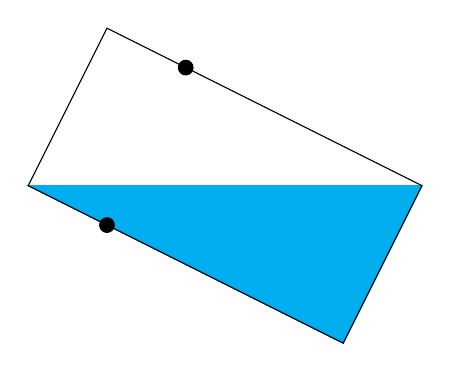
\begin{tikzpicture}
			\draw[fill,color=cyan] (0,0) -- (4,-2) -- (5,0) -- cycle;
			\path[draw] (0,0) -- (1,2) -- (5,0) -- (4,-2) -- cycle;
			\fill[black] (1,-0.5) circle[radius=0.1];
			\fill[black] (2,1.5) circle[radius=0.1];
		\end{tikzpicture}
		\caption{Кастрюля}
	\end{minipage}
	\begin{minipage}{0.48\textwidth}\centering
		
\begin{tikzpicture}
			\rectangle{0}{0}{2}{0.5}
			\rectangle{2.5}{0}{1}{0.5}
			\rectangle{0}{1}{1.5}{0.5}
			\rectangle{2}{1}{1.5}{0.5}
			\rectangle{0}{2}{1}{0.5}
			\rectangle{1.5}{2}{1}{0.5}
			\rectangle{0}{3}{0.5}{0.5}
			\rectangle{1}{3}{0.5}{0.5}
			\rectangle{2}{3}{0.5}{0.5}
			\rectangle{3}{3}{0.5}{0.5}
			\draw[step=0.5,thin,black!60] (0,0) grid (3.5,3.5);
		\end{tikzpicture}
		\caption{Корабли на поле $7\times7$}
	\end{minipage}
\end{figure}

\end{document}
